\chapter{Cloud Environment and Central Monitoring Foundation}

\section{Introduction}

ARIA does not generate telemetry by itself; it consumes telemetry that already exists in Elasticsearch. Before any intelligence can be built, that telemetry must actually arrive: real host, network, runtime, and resource events must be produced, forwarded, indexed, and made queryable.

This chapter follows the engineering story at its foundation. It covers:

\begin{itemize}[leftmargin=1cm]
\item the Huawei Cloud environment that hosts the stack;
\item the preparation and hardening of the central server;
\item the network, ports, and communication design;
\item the installation, configuration, and automation of each monitoring and security tool;
\item the verification that real data is present inside Elasticsearch.
\end{itemize}

The chapter ends with live Elasticsearch evidence, which is the precondition for everything ARIA does in the following chapters.

\section{Huawei Cloud Environment}

The monitoring and intelligence stack was hosted on a Huawei Cloud environment provisioned through the academic cloud console. The environment groups a Virtual Private Cloud (VPC), a subnet, a security group, an Elastic IP (EIP), and an Elastic Cloud Server (ECS) virtual machine. The stated objective was to host the SOC stack in a controlled environment with sufficient compute, memory, storage, and network isolation.

\diagramimagecompact{phase2_huawei_cloud_environment.png}{Huawei Cloud environment used for the project}

The central host is an ECS instance named \codepath{ecs-ghazi} running Ubuntu~24, sized with a large flavor (64~vCPUs and 128~GB of memory) so that Elasticsearch, Kibana, Wazuh, Suricata, Falco/Falcosidekick, Telegraf, Redis, and the ARIA backend can run together on a single node during the internship. Figure~\ref{fig:cloud-ecs} shows the ECS summary of this host, and Figure~\ref{fig:cloud-vpc} shows the VPC topology in which it is deployed. The security-group and Elastic IP console views are reproduced as cloud evidence in Appendix~\ref{app:cloud}.

\begin{figure}[H]
\centering
\fbox{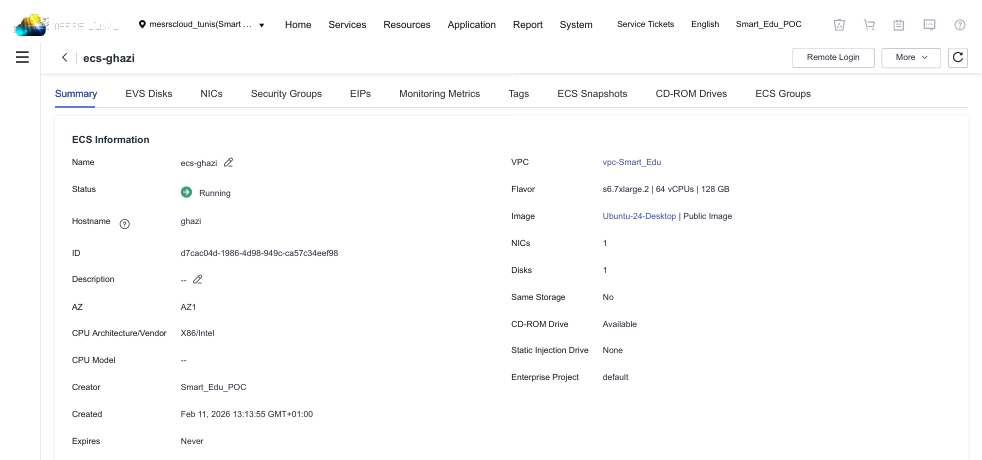
\includegraphics[width=0.96\textwidth,height=0.40\textheight,keepaspectratio]{assets/cloud/cloud_ecs.png}}
\caption{Central ECS host (\texttt{ecs-ghazi}) running the SOC and ARIA stack}
\label{fig:cloud-ecs}
\end{figure}

\begin{figure}[H]
\centering
\fbox{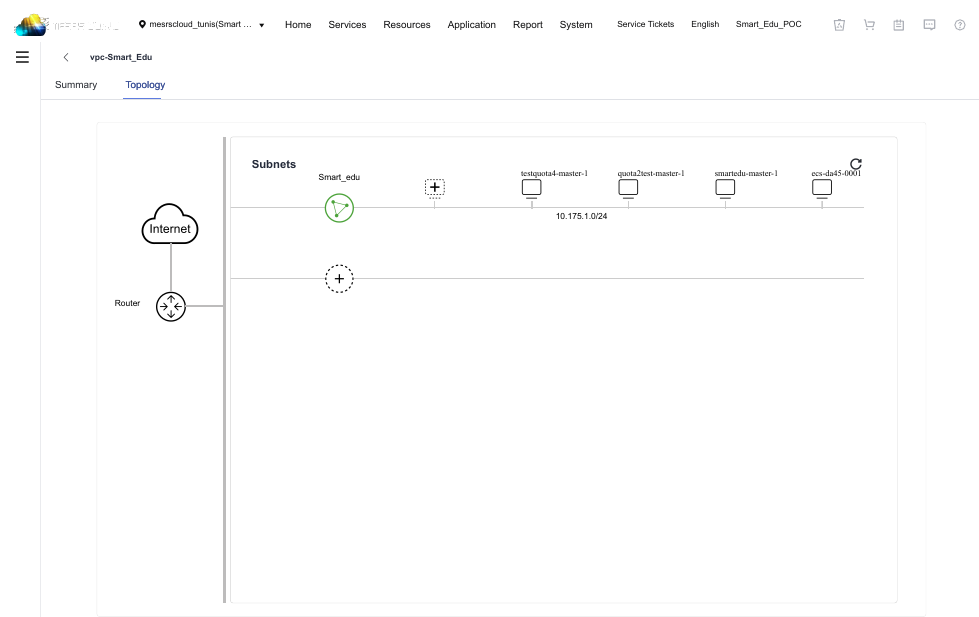
\includegraphics[width=0.96\textwidth,height=0.32\textheight,keepaspectratio]{assets/cloud/cloud_vpc.png}}
\caption{Virtual Private Cloud topology hosting the monitoring environment}
\label{fig:cloud-vpc}
\end{figure}

\section{Main Server Preparation}

The central server is the single node on which the whole monitoring foundation is installed. Its preparation followed a deliberate order so that later components could rely on a stable base:

\begin{enumerate}[leftmargin=1cm]
\item \textbf{Base utilities.} Operating-system package sources were fixed and updated, and the utilities required by the setup scripts (\codepath{curl}, \codepath{gpg}, \codepath{wget}, \codepath{tar}, \codepath{ca-certificates}, \codepath{unzip}) were installed.
\item \textbf{Central address.} The local IP address of the host was detected and reused consistently as the binding and connection address for every service, so that Elasticsearch, Kibana, Filebeat, Falcosidekick, and Telegraf all agree on the same central endpoint.
\item \textbf{Hardening.} The host was hardened (Section~\ref{sec:stability}) before exposing any service.
\end{enumerate}

This ordering matters: a service installed before the firewall and SSH policy are in place would be briefly exposed, and a service bound to the wrong address would silently fail to receive data.

Figure~\ref{fig:deployment-context} summarizes the resulting deployment: the single Ubuntu host runs the security and observability tools partly as native system services (Suricata, Wazuh Manager, Filebeat, Telegraf, Elasticsearch, and Kibana) and partly as Docker services (Falco and Falcosidekick), with the main configuration files and the hardware requirements that the host must satisfy.

\begin{figure}[H]
\centering
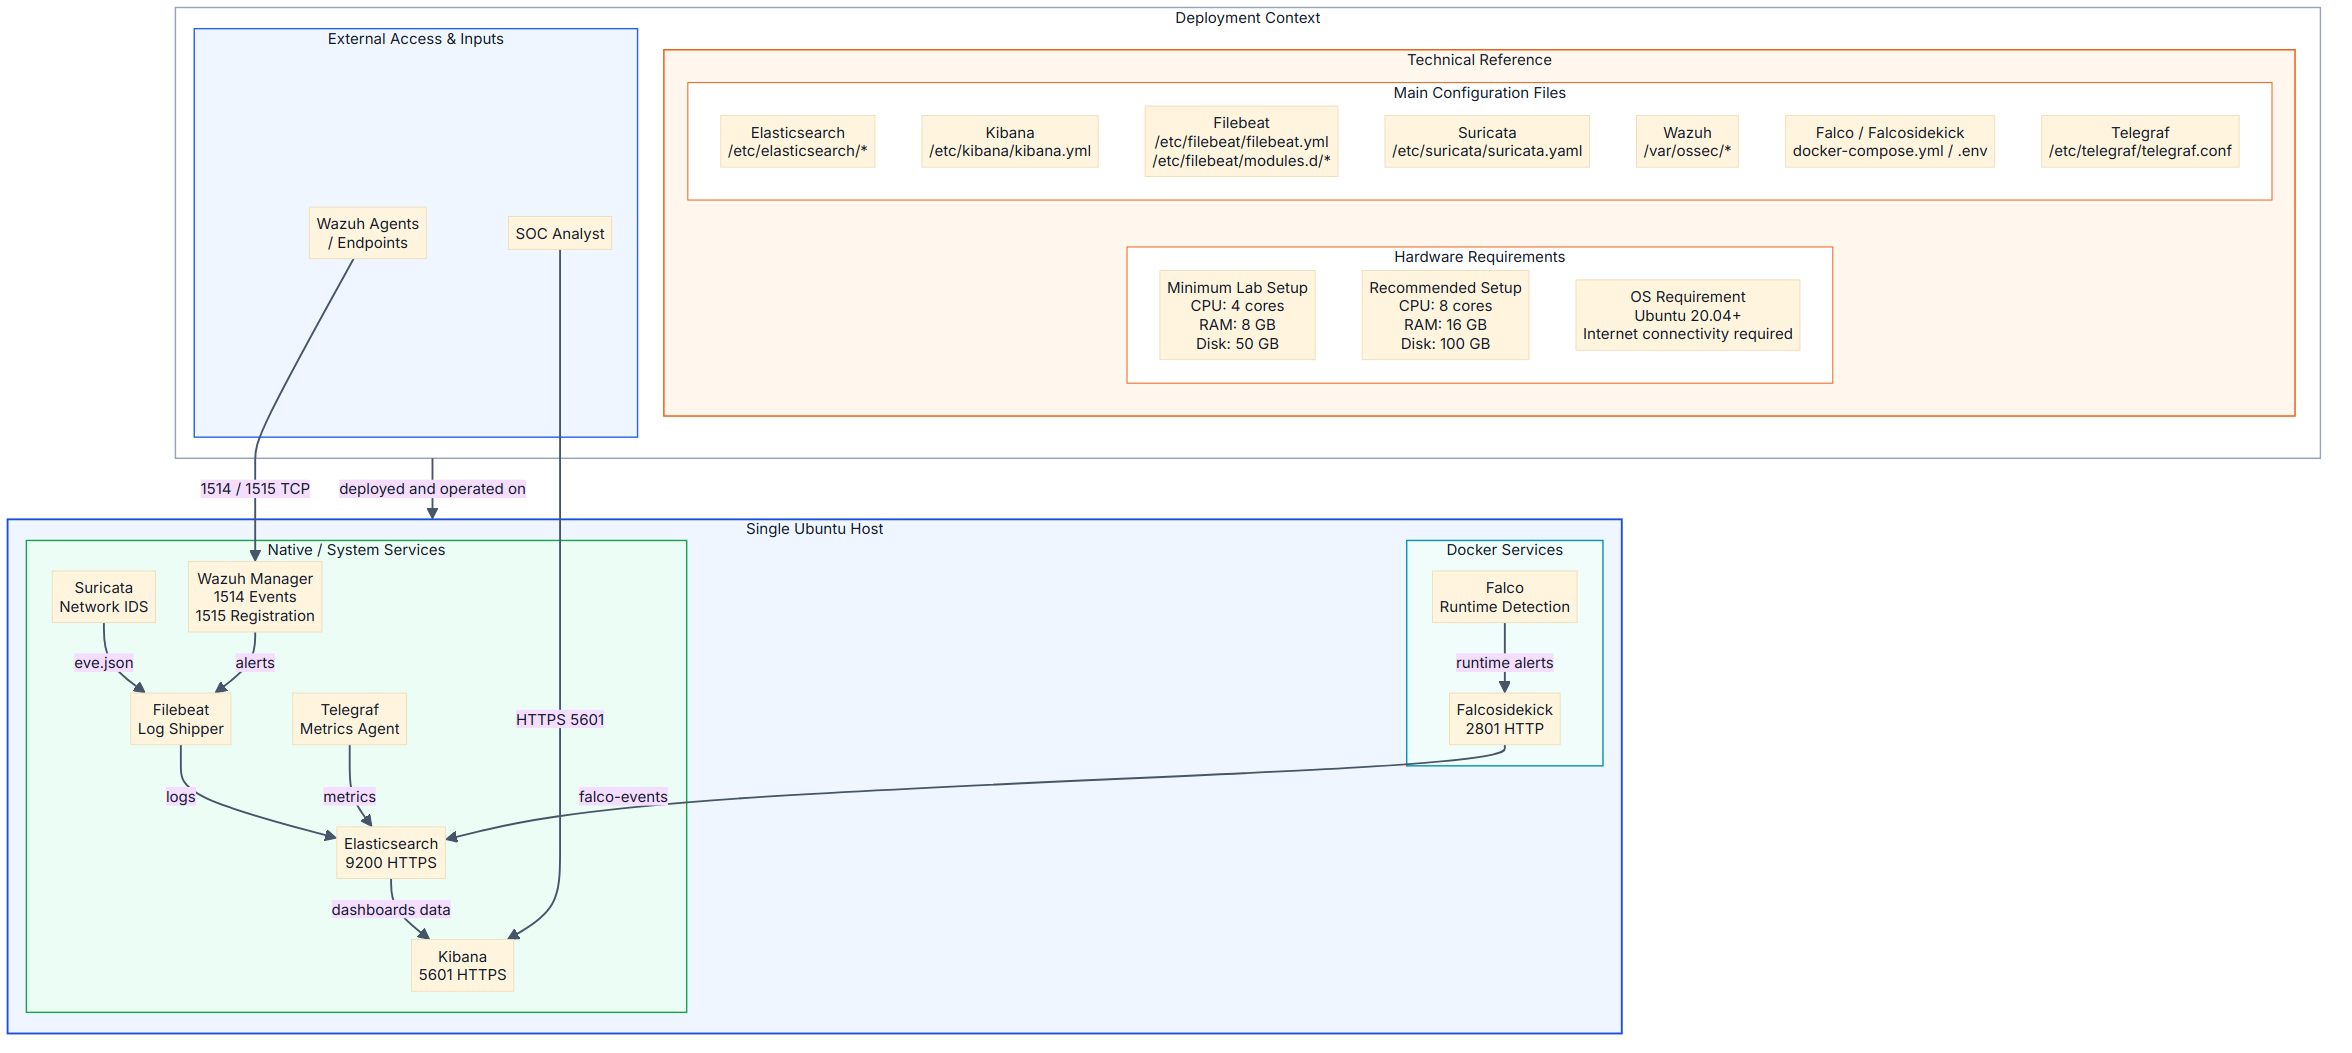
\includegraphics[width=\textwidth,height=0.42\textheight,keepaspectratio]{assets/diagrams/phase1_deployment_requirements.png}
\caption{Deployment context, services, configuration files, and host requirements}
\label{fig:deployment-context}
\end{figure}

\section{Network, Ports, and Communication}

The central host is reachable from the outside only through its Elastic IP, and the security group is the main network control between that public address and the internal services. The design principle is restrictive exposure: only the ports strictly required for monitoring agents and analysts are opened, and everything else is denied by default.

\begin{table}[H]
\centering
\caption{Central stack network ports}
\begin{tabularx}{\textwidth}{@{}p{0.16\textwidth}p{0.20\textwidth}Y@{}}
\toprule
\textbf{Port} & \textbf{Service} & \textbf{Purpose and exposure} \\
\midrule
9200/tcp & Elasticsearch & TLS-secured ingest and query endpoint used by Filebeat, Falcosidekick, Telegraf, and the ARIA backend. \\
5601/tcp & Kibana & Analyst web interface for search and visualization; should be restricted to analysts or VPN. \\
1514/tcp,udp & Wazuh Manager & Reception of Wazuh Agent security events from monitored servers. \\
1515/tcp & Wazuh Manager & Wazuh Agent enrollment (registration) channel. \\
55000/tcp & Wazuh API & Wazuh management API used to query agents and rules. \\
2801/tcp & Falcosidekick & Reception/forwarding endpoint for Falco runtime events. \\
22/tcp & SSH & Administrative access, hardened and restricted to trusted networks. \\
\bottomrule
\end{tabularx}
\end{table}

All forwarding toward Elasticsearch uses HTTPS with the cluster certificate authority, and the security accounts (\codepath{elastic}, \codepath{kibana}, and the beats/monitoring users) are created during installation. SSH access should be limited to administrative networks, Kibana should be restricted to analysts or VPN access, Elasticsearch should remain internal, and Wazuh/Falco ports should only be exposed where required by monitored agents.

\section{Central Monitoring Stack Architecture}

The central stack is a layered pipeline. Detection and collection tools run on monitored hosts and on the central server, forwarders ship their output to Elasticsearch, Elasticsearch indexes and stores the data, Kibana provides direct exploration, and Redis supports the ARIA workflow that is built on top. Figure~\ref{fig:central-stack} shows how the tools combine into a single ingestion path that ends in Elasticsearch indices, which are the data contract consumed by ARIA.

\begin{figure}[H]
\centering
\begin{adjustbox}{max width=\textwidth}\begin{tikzpicture}[
  font=\small,
  src/.style={draw, rounded corners, align=center, text width=2.6cm, minimum height=1.5cm, fill=gray!8, font=\fontsize{10}{12}\selectfont},
  fwd/.style={draw, rounded corners, align=center, text width=2.5cm, minimum height=1.5cm, fill=teal!10, font=\fontsize{10}{12}\selectfont},
  store/.style={draw, cylinder, shape border rotate=90, aspect=0.25, align=center, text width=2.8cm, minimum height=1.7cm, fill=blue!8, font=\fontsize{10}{12}\selectfont},
  app/.style={draw, rounded corners, align=center, text width=2.6cm, minimum height=1.5cm, fill=orange!10, font=\fontsize{10}{12}\selectfont},
  group/.style={draw=none, rounded corners=4pt, inner sep=10pt, opacity=0.25},
  arrow/.style={-Latex, line width=1.1pt},
  logopic/.style={inner sep=0pt}
]
% Source nodes
\node[src] (wazuh) {
\includegraphics[width=0.8cm]{assets/logos/wazuh.png}\\[2pt]\textbf{Wazuh}\\host security};
\node[src, below=0.35cm of wazuh] (suricata) {
\includegraphics[width=0.8cm]{assets/logos/suricata.png}\\[2pt]\textbf{Suricata}\\network IDS};
\node[src, below=0.35cm of suricata] (falco) {
\includegraphics[width=0.8cm]{assets/logos/falco.png}\\[2pt]\textbf{Falco}\\runtime security};
\node[src, below=0.35cm of falco] (telegraf) {
\includegraphics[width=0.8cm]{assets/logos/influxdb.png}\\[2pt]\textbf{Telegraf}\\metrics};

% Forwarder
\node[fwd, right=1.2cm of suricata] (filebeat) {
\includegraphics[width=0.8cm]{assets/logos/filebeat.png}\\[2pt]\textbf{Filebeat}\\+ Falcosidekick};

% Store
\node[store, right=1.2cm of filebeat, yshift=-0.5cm] (es) {
\includegraphics[width=0.8cm]{assets/logos/elasticsearch.png}\\[2pt]\textbf{Elasticsearch}\\indices};

% App nodes
\node[app, above=0.9cm of es] (kibana) {
\includegraphics[width=0.8cm]{assets/logos/elasticstack.png}\\[2pt]\textbf{Kibana}\\explore};
\node[app, right=1.2cm of es] (aria) {
\includegraphics[width=0.8cm]{assets/logos/aria-logo-transparent.png}\\[2pt]\textbf{ARIA}\\backend};
\node[store, below=0.9cm of aria] (redis) {
\includegraphics[width=0.8cm]{assets/logos/redis.png}\\[2pt]\textbf{Redis}\\cache/cursors};

% Group backgrounds (after nodes exist)
\node[group, fill=gray!30, fit={(wazuh) (telegraf)}] (gsrc) {};
\node[group, fill=teal!30, fit={(filebeat)}] (gfwd) {};
\node[group, fill=blue!30, fit={(es)}] (gstore) {};
\node[group, fill=orange!30, fit={(kibana) (aria) (redis)}] (gapp) {};

% Arrows
\draw[arrow] (wazuh) -- (filebeat);
\draw[arrow] (suricata) -- (filebeat);
\draw[arrow] (falco) -- (filebeat);
\draw[arrow] (telegraf.east) -- (es.west);
\draw[arrow] (filebeat) -- (es);
\draw[arrow] (es) -- (kibana);
\draw[arrow] (es) -- (aria);
\draw[arrow] (redis) -- (aria);

% Group labels
\node[font=\fontsize{11}{13}\selectfont\bfseries, text=gray!70!black, above=0.2cm of gsrc.north west, anchor=west] {Sources};
\node[font=\fontsize{11}{13}\selectfont\bfseries, text=teal!70!black, above=0.2cm of gfwd.north west, anchor=west] {Forwarders};
\node[font=\fontsize{11}{13}\selectfont\bfseries, text=blue!70!black, above=0.2cm of gstore.north west, anchor=west] {Store};
\node[font=\fontsize{11}{13}\selectfont\bfseries, text=orange!70!black, above=0.2cm of gapp.north west, anchor=west] {Consumers};
\end{tikzpicture}\end{adjustbox}
\caption{Central monitoring stack architecture and ingestion path}
\label{fig:central-stack}
\end{figure}

Seen as a data-flow, the same stack is Figure~\ref{fig:df-monitoring}: each kind of signal on a monitored host (OS and authentication logs, network packets, runtime syscalls, and system metrics) is captured by a dedicated tool, carried by the right forwarder (Wazuh Manager, Filebeat, Falcosidekick, or Telegraf directly), and deposited into a predictable Elasticsearch index family, which the ARIA poller then reads. Figure~\ref{fig:deploy-full} places these same components on the physical deployment: the Huawei Cloud VPC, the ECS node that hosts both the ARIA application and the central stack, the labelled ports, and the monitored servers reached over the network.

\umlfigure{monitoring_data_flow.png}{Monitoring data-flow from monitored host to Elasticsearch indices}{fig:df-monitoring}

\umlfigure{cloud_deployment_diagram.png}{Deployment diagram of the cloud environment, central stack, and monitored servers}{fig:deploy-full}

The installation of the stack is driven by a set of setup scripts. A small wrapper script, \sourcefile{setup_script.sh}, delegates to the maintained orchestrator \sourcefile{setup_script_telegraf.sh}, which installs the selected components through command-line flags. The following sections describe each tool, the configuration logic applied, and the data it produces. Section~\ref{sec:setup-automation} then explains the automation and ordering that the orchestrator enforces.

\section{Elasticsearch and Kibana}

\raisebox{-0.22cm}{
\includegraphics[width=1.0cm]{assets/logos/elasticsearch.png}}\hspace{0.15cm}Elasticsearch is the central indexing, search, and storage engine; \raisebox{-0.22cm}{
\includegraphics[width=1.0cm]{assets/logos/elasticstack.png}}\hspace{0.15cm}Kibana is its visualization front end. They are installed together by \sourcefile{siem_setup.sh} from the official Elastic 7.x APT repository at a pinned version, so that every component of the stack agrees on a single compatible release.

The configuration logic is security-first. Elasticsearch is configured as a single-node cluster (\codepath{discovery.type: single-node}) that binds to all interfaces on port~9200, with \codepath{xpack.security.enabled} turned on and TLS enabled on both the transport and HTTP layers. The certificates are generated locally with \codepath{elasticsearch-certutil}, which produces a certificate authority and per-service certificates for Elasticsearch, Kibana, and Filebeat; these are installed under each service's \codepath{certs} directory with restrictive ownership and permissions. After the service starts, the built-in users (\codepath{elastic}, \codepath{kibana}, \codepath{beats_system}, and the monitoring users) receive passwords through \codepath{elasticsearch-setup-passwords}. This means that from the very first component, no traffic and no authentication is left in clear text.

\begin{table}[H]
\centering
\caption{Key Elasticsearch and Kibana configuration choices}
\begin{tabularx}{\textwidth}{@{}p{0.30\textwidth}Y@{}}
\toprule
\textbf{Setting} & \textbf{Reasoning} \\
\midrule
\codepath{discovery.type: single-node} & The whole stack runs on one ECS host during the internship; single-node mode avoids cluster bootstrap complexity. \\
\codepath{network.host: 0.0.0.0}, \codepath{http.port: 9200} & The service must be reachable by Filebeat, Falcosidekick, Telegraf, and ARIA; exposure is then constrained by the firewall. \\
\codepath{xpack.security.enabled: true} + TLS & Authentication and encryption are mandatory because the index stores sensitive security events. \\
Local CA via \codepath{elasticsearch-certutil} & A self-managed CA secures transport and HTTP without depending on external certificate infrastructure. \\
Kibana \codepath{server.port: 5601}, TLS, \codepath{elasticsearch.username: elastic} & Kibana connects to Elasticsearch over HTTPS and serves the analyst UI over TLS. \\
\bottomrule
\end{tabularx}
\end{table}

Kibana is configured to reach Elasticsearch over HTTPS using the generated certificate authority and the \codepath{elastic} account, serves its own interface over TLS on port~5601, and is given an encryption key for its saved objects. Once both services are enabled and started through \codepath{systemd}, the operator has a working, secured search and visualization core on which all other tools deposit their data.

\section{Wazuh}

\raisebox{-0.22cm}{
\includegraphics[width=1.1cm]{assets/logos/wazuh.png}}\hspace{0.15cm}Wazuh provides host and endpoint security monitoring: it analyzes authentication events, file integrity, rootcheck results, and system activity, and raises rule-based security alerts. On the central server, \sourcefile{wazuh_setup.sh} installs the \textbf{Wazuh Manager} from the Wazuh 4.x APT repository at the pinned version \codepath{wazuh-manager=4.5.4-1}, then enables and starts it through \codepath{systemd}.

The important integration step is connecting Wazuh to the rest of the stack. The script appends a Wazuh module block to the Filebeat configuration so that Wazuh alerts are read and shipped into Elasticsearch under the \codepath{wazuh-alerts-*} index family. This is the bridge that turns Wazuh from a stand-alone manager into a source that ARIA can poll: every security alert the manager produces becomes a document in a predictable index pattern. The manager also exposes its API on port~55000 and receives agent events on ports~1514/1515, which become relevant in Chapter~5 when monitored servers enroll their Wazuh Agents.

\section{Suricata}

\raisebox{-0.22cm}{
\includegraphics[width=1.1cm]{assets/logos/suricata.png}}\hspace{0.15cm}Suricata is the network intrusion detection engine. It inspects traffic on a network interface and emits structured security events. On the central host, \sourcefile{suricata_setup.sh} installs Suricata from the official OISF stable PPA together with its capture dependencies, then performs a key piece of automation: it detects the active network interface from the default route (\codepath{ip route show default}) and writes it into both \codepath{/etc/default/suricata} and the rendered configuration. This avoids the most common Suricata misconfiguration, which is listening on the wrong interface and therefore seeing no traffic.

The configuration itself is rendered from the \sourcefile{suricata_temp.yaml} template. The template defines the protected network ranges through \codepath{HOME_NET} (the RFC~1918 private ranges) versus \codepath{EXTERNAL_NET}, and enables the \codepath{eve-log} output that writes events as JSON to \codepath{eve.json}. The EVE JSON output is what makes Suricata consumable downstream: Filebeat ships these JSON events into Elasticsearch, where ARIA's Suricata mapper interprets them as network alerts. After the configuration is applied, the service is restarted and the script confirms startup by checking for the ``Engine started'' marker in the Suricata log.

\section{Falco and Falcosidekick}

\raisebox{-0.22cm}{
\includegraphics[width=1.1cm]{assets/logos/falco.png}}\hspace{0.15cm}Falco provides runtime security: it watches system calls and container behavior and raises events when something abnormal happens, such as a shell launched inside a container or a sensitive file being read. On the central server, \sourcefile{setup-falco-server-elastic.sh} installs Falco from the official Falco security APT repository and selects the modern eBPF driver service (\codepath{falco-modern-bpf.service}) so that Falco works on a current kernel without building a kernel module.

Falco on its own only prints events; the forwarding to Elasticsearch is performed by \textbf{Falcosidekick}. The script configures Falcosidekick with the central Elasticsearch URL (\codepath{https://<host>:9200}), the \codepath{elastic} credentials, and a target index prefix (\codepath{falco-events-server} on the central node, and a per-server prefix on monitored hosts). Before reconfiguring anything, the script backs up and removes any previous Docker-based Falco deployment so that the new server-side forwarding configuration is authoritative. It also validates the Elasticsearch endpoint before continuing, which prevents Falcosidekick from being started against an unreachable or misauthenticated target. The result is a runtime-event index family that ARIA's runtime investigation engine consumes in Chapter~4.

\section{Filebeat}

\raisebox{-0.22cm}{
\includegraphics[width=1.1cm]{assets/logos/filebeat.png}}\hspace{0.15cm}Filebeat is the log-forwarding layer of the stack. It is installed together with Elasticsearch and Kibana by \sourcefile{siem_setup.sh}, shares the same certificate authority, and ships system and authentication logs into Elasticsearch. Two roles make Filebeat central to the architecture. First, it carries Wazuh alerts through the Wazuh module added during the Wazuh setup, producing the \codepath{wazuh-alerts-*} indices. Second, on monitored servers it carries Suricata EVE JSON and system logs into per-server \codepath{filebeat-<asset>-*} indices. Because so many sources travel through Filebeat, its TLS configuration and index naming directly determine what ARIA can later query and how it scopes data by server. Listing~\ref{lst:filebeat} shows the essential output block: Filebeat ships over HTTPS to Elasticsearch on port~9200, authenticates as a beats user, and trusts the locally generated cluster CA, with the password masked.

\begin{lstlisting}[style=aria,language=yaml,caption={Filebeat Elasticsearch output (sanitized excerpt)},label={lst:filebeat}]
output.elasticsearch:
  hosts: ["https://<central-host>:9200"]
  protocol: "https"
  username: "filebeat_writer"
  password: "******"
  ssl.certificate_authorities: ["/etc/filebeat/certs/ca.crt"]
  ssl.verification_mode: "full"
\end{lstlisting}

\section{Telegraf}

\raisebox{-0.22cm}{
\includegraphics[width=1.1cm]{assets/logos/influxdb.png}}\hspace{0.15cm}Telegraf is the metrics agent. It collects infrastructure metrics such as CPU, memory, disk, network, load, processes, and sockets, and writes them to Elasticsearch. On the central host, \sourcefile{telegraf_setup.sh} installs Telegraf from the InfluxData repository and configures an Elasticsearch output rather than the default InfluxDB output, because in this project Elasticsearch is the single shared store for both security events and metrics.

The configuration logic is careful about two practical issues. First, Telegraf must trust the Elasticsearch certificate authority, so the script installs the cluster CA into a dedicated, group-readable \codepath{certs} directory owned by the \codepath{telegraf} user. Second, it detects the Elasticsearch version before writing the output block, because the Elasticsearch output behaves differently across versions; if the version cannot be detected, the script stops rather than producing a silently broken metrics pipeline. A small custom input is also added to report the size of selected directories, which complements the standard host metrics. Telegraf writes into \codepath{telegraf-*} indices, which feed the metrics dashboard and the infrastructure investigations described in Chapter~4. Listing~\ref{lst:telegraf} shows the Elasticsearch output that replaces the default InfluxDB sink.

\begin{lstlisting}[style=aria,language=conf,caption={Telegraf Elasticsearch output (sanitized excerpt)},label={lst:telegraf}]
[[outputs.elasticsearch]]
  urls = ["https://<central-host>:9200"]
  username = "telegraf_writer"
  password = "******"
  index_name = "telegraf-%Y.%m.%d"
  tls_ca = "/etc/telegraf/certs/ca.crt"
  insecure_skip_verify = false
  manage_template = false
\end{lstlisting}

\section{Redis and Supporting Services}

\raisebox{-0.22cm}{
\includegraphics[width=1.0cm]{assets/logos/redis.png}}\hspace{0.15cm}Redis is not a detection tool but a supporting service for the ARIA workflow. It provides a low-latency store for polling cursors, deduplication keys, rolling metric baselines, retry queues, and cached performance data. Keeping this operational state in Redis, rather than recomputing it from Elasticsearch on every cycle, is what allows ARIA's pipeline to poll incrementally and avoid reprocessing the same events. Redis runs locally on the central host alongside the rest of the stack and is reached only by the ARIA backend; it is never exposed to monitored servers or to the public network.

\section{Setup Scripts and Automation Logic}
\label{sec:setup-automation}

The whole foundation is reproducible because it is expressed as scripts rather than manual steps. The orchestrator \sourcefile{setup_script_telegraf.sh} exposes per-component flags, so an operator can install or reinstall only the parts that are needed instead of rebuilding the whole node. Each component script is idempotent in spirit: it detects an existing installation, optionally removes it cleanly, installs a pinned version, writes its configuration, enables the service, and verifies that it started.

\begin{table}[H]
\centering
\caption{Central setup script inventory}
\begin{tabularx}{\textwidth}{@{}p{0.30\textwidth}Y@{}}
\toprule
\textbf{Script or config} & \textbf{Purpose} \\
\midrule
\sourcefile{setup_script.sh} and \sourcefile{setup_script_telegraf.sh} & Orchestrate central stack installation through component flags. \\
\sourcefile{siem_setup.sh} & Install and configure Elasticsearch, Kibana, Filebeat, TLS material, service startup, and system log forwarding. \\
\sourcefile{wazuh_setup.sh} & Install Wazuh Manager (4.5.4-1) and integrate Wazuh alerts into Filebeat. \\
\sourcefile{suricata_setup.sh} and \sourcefile{suricata_temp.yaml} & Configure Suricata IDS capture, interface detection, and EVE JSON output. \\
\sourcefile{setup-falco-server-elastic.sh} & Configure Falco and Falcosidekick server-side forwarding to Elasticsearch. \\
\sourcefile{telegraf_setup.sh} and Telegraf configs & Configure infrastructure metric collection and forwarding to Elasticsearch. \\
\sourcefile{detection_rules_setup.sh} & Import detection rules and saved objects into the visualization stack. \\
\sourcefile{hardening_setup.sh} & Apply host hardening: Fail2Ban, UFW firewall, and SSH hardening. \\
\bottomrule
\end{tabularx}
\end{table}

The automation enforces a deliberate ordering. The search core (Elasticsearch and Kibana) is installed first because every other component forwards to it. Wazuh follows because it reuses Filebeat. Suricata, Falco, and Telegraf are then added as independent sources. Detection rules and saved objects are imported last, once Kibana is available. These scripts are provisioning scripts that can install, reconfigure, or replace services; their role in this report is environment-preparation evidence, and they should be reviewed before being run on an existing server rather than executed blindly. Figure~\ref{fig:act-central} captures this ordering as an activity diagram, from the root/OS pre-checks and local-IP detection, through the search core, security tools, forwarders, and hardening, to the final service-health and telemetry checks.

\umlfigure{act_central_setup.png}{Central setup script activity flow}{fig:act-central}

\section{Stability, Service Checks, and Hardening}
\label{sec:stability}

A monitoring foundation is only useful if it stays up and is not itself a soft target. Two mechanisms address this. The first is built into every component script: after enabling a service, the script verifies with \codepath{systemctl is-active} (and, for Suricata, a log marker) that the service actually started, and reports clearly when it did not. This turns a silent failure into a visible one during installation.

The second mechanism is host hardening, applied by \sourcefile{hardening_setup.sh}, which performs three actions. It installs and enables \textbf{Fail2Ban} with an \codepath{sshd} jail (five retries, one-hour ban) to slow down brute-force attempts. It installs and configures the \textbf{UFW} firewall with a default-deny inbound policy and explicit allow rules only for the stack ports (SSH, 5601, 9200, 1514, 1515, 55000), optionally restricted to a trusted CIDR. And it hardens \textbf{SSH} by disabling root login and password authentication, enabling public-key authentication, lowering \codepath{MaxAuthTries} to three, and setting client-alive limits. Together these checks and controls keep the foundation both running and defensible.

\begin{table}[H]
\centering
\caption{Host hardening actions}
\begin{tabularx}{\textwidth}{@{}p{0.22\textwidth}Y@{}}
\toprule
\textbf{Control} & \textbf{Configuration applied} \\
\midrule
Fail2Ban & \codepath{sshd} jail enabled, \codepath{maxretry = 5}, \codepath{bantime = 3600}. \\
UFW firewall & Default deny incoming, allow outgoing; explicit allow for 22, 5601, 9200, 1514, 1515, 55000, optionally scoped to \codepath{ARIA_ALLOWED_CIDR}. \\
SSH hardening & \codepath{PermitRootLogin no}, \codepath{PasswordAuthentication no}, \codepath{PubkeyAuthentication yes}, \codepath{MaxAuthTries 3}, client-alive limits, no empty passwords. \\
\bottomrule
\end{tabularx}
\end{table}

\section{Validation of Tool Installation}

Installation is not complete until each service is confirmed active. The natural validation command is a single \codepath{systemctl status} over the full set of central services, which proves at a glance that the foundation is running:

\begin{center}
\codepath{systemctl status elasticsearch kibana filebeat wazuh-manager suricata falcosidekick telegraf fail2ban}
\end{center}

Each service must report an active state. Because the setup scripts already check startup during installation, this command is mostly a post-installation confirmation and a routine health check that an operator can repeat at any time. The configuration-derived service matrix and the live Kibana/Elasticsearch evidence that independently confirm these services are operational are presented in the validation chapter (Section~\ref{sec:val-es} and Table~\ref{tab:svc-matrix}).

\section{Elasticsearch Data Verification}

The decisive test of the whole foundation is not that the services run, but that real data has arrived in Elasticsearch. Once the tools are active, each source creates and fills its own index family, and a simple authenticated index listing (with credentials hidden) shows documents accumulating. The index families produced by the foundation are the data contract that ARIA depends on:

\begin{table}[H]
\centering
\caption{Index families produced by the monitoring foundation}
\begin{tabularx}{\textwidth}{@{}p{0.20\textwidth}p{0.28\textwidth}Y@{}}
\toprule
\textbf{Source} & \textbf{Index family} & \textbf{Content used by ARIA} \\
\midrule
Wazuh & \codepath{wazuh-alerts-*} & Host security alerts, rules, authentication, integrity findings. \\
Suricata & \codepath{filebeat-*} (EVE JSON) & Network IDS events and IP context. \\
Falco & \codepath{falco-*} & Runtime security events for runtime investigations. \\
Filebeat & \codepath{filebeat-*} & System and authentication logs. \\
Telegraf & \codepath{telegraf-*} & CPU, memory, disk, network, process, and socket metrics. \\
\bottomrule
\end{tabularx}
\end{table}

Figure~\ref{fig:ch2-es-idx} is a live Elasticsearch index-management capture showing these index families populated for both the central host and a monitored asset, with real document counts, storage sizes, and health states. The presence of these documents is exactly the precondition the next chapter assumes: from here on, ARIA can poll real indices rather than empty ones. Additional index pages and a live Kibana \emph{Discover} view are reproduced in the validation chapter (Section~\ref{sec:val-es}) and Appendix~\ref{app:cloud-es}.

\screenshot{aria_es_indices1.png}{Live Elasticsearch index management: Wazuh, Filebeat, Falco, and Telegraf index families with real document counts, storage sizes, and health states}{fig:ch2-es-idx}

\section{Conclusion}

This chapter built the foundation of the solution: a Huawei Cloud environment hosting a hardened central server, and a complete monitoring stack in which Elasticsearch, Kibana, Wazuh, Suricata, Falco/Falcosidekick, Filebeat, Telegraf, and Redis are installed and configured by reproducible scripts, kept stable by service checks and host hardening, and verified to deliver real telemetry into Elasticsearch. With genuine data now present and queryable, the next chapter turns to the platform that gives this data operational meaning: the design and internal logic of ARIA.
